\documentclass[14pt,a4paper]{article}

\usepackage{textgreek}
\usepackage[utf8x]{inputenc}
\usepackage{graphicx}
\usepackage[export]{adjustbox}
\usepackage[a4paper, portrait, margin=1in]{geometry}
\usepackage[ukrainian]{babel}
\usepackage{cmap}
\usepackage{etoolbox}
\usepackage{caption}
\usepackage{booktabs}
\usepackage{listings}
\usepackage{pgfplots}
\usepackage{xcolor} 
\usepackage{titlesec}
\usepackage{setspace}
\usepackage{fancyhdr} 
\usepackage{amsmath} 
\usepackage{amsthm}
\usepackage{hyperref}
\usepackage{amsmath} 
\usepackage{bm} 
\usepackage[square,sort,comma,numbers,super]{natbib}
\usepackage{caption}
\usepackage{float}

\graphicspath{ {./Images/} }

\title{\Huge \textbf{Інструкція до інсталяції та конфігурування системи AtOM. Access to Memory} }
\date{}

\begin{document}

\begin{titlepage}
    \pagecolor{green} 
    \color{black}
    \maketitle
    \thispagestyle{empty}
    
	\begin{center}
	
\includegraphics[max width=1.5\textwidth]{Images/logo_grn.png}
	\end{center}    
    
    \vspace*{8cm}
    \center \textbf{Львівський національний університет імені Івана Франка}
    \center \textbf{Львів 2024}

\end{titlepage}

\pagecolor{white}
\color{black}

\newpage

\pagenumbering{Roman}
\tableofcontents
\newpage
\pagenumbering{arabic}

\section{Загальна інформація}
\begin{large}
\textbf{AtoM} визначається як \textbf{"Access to Memory"}. Це є веб-програма з відкритим вихідним для архівного опису та доступу на основі стандартів у багатомовному середовищі з \textbf{мультирепозитарною системою}, тобто такою, яка використовується мережею архівних установ або інших типів сховищ.

\subsection{Технічний огляд}
    
	\begin{center}
	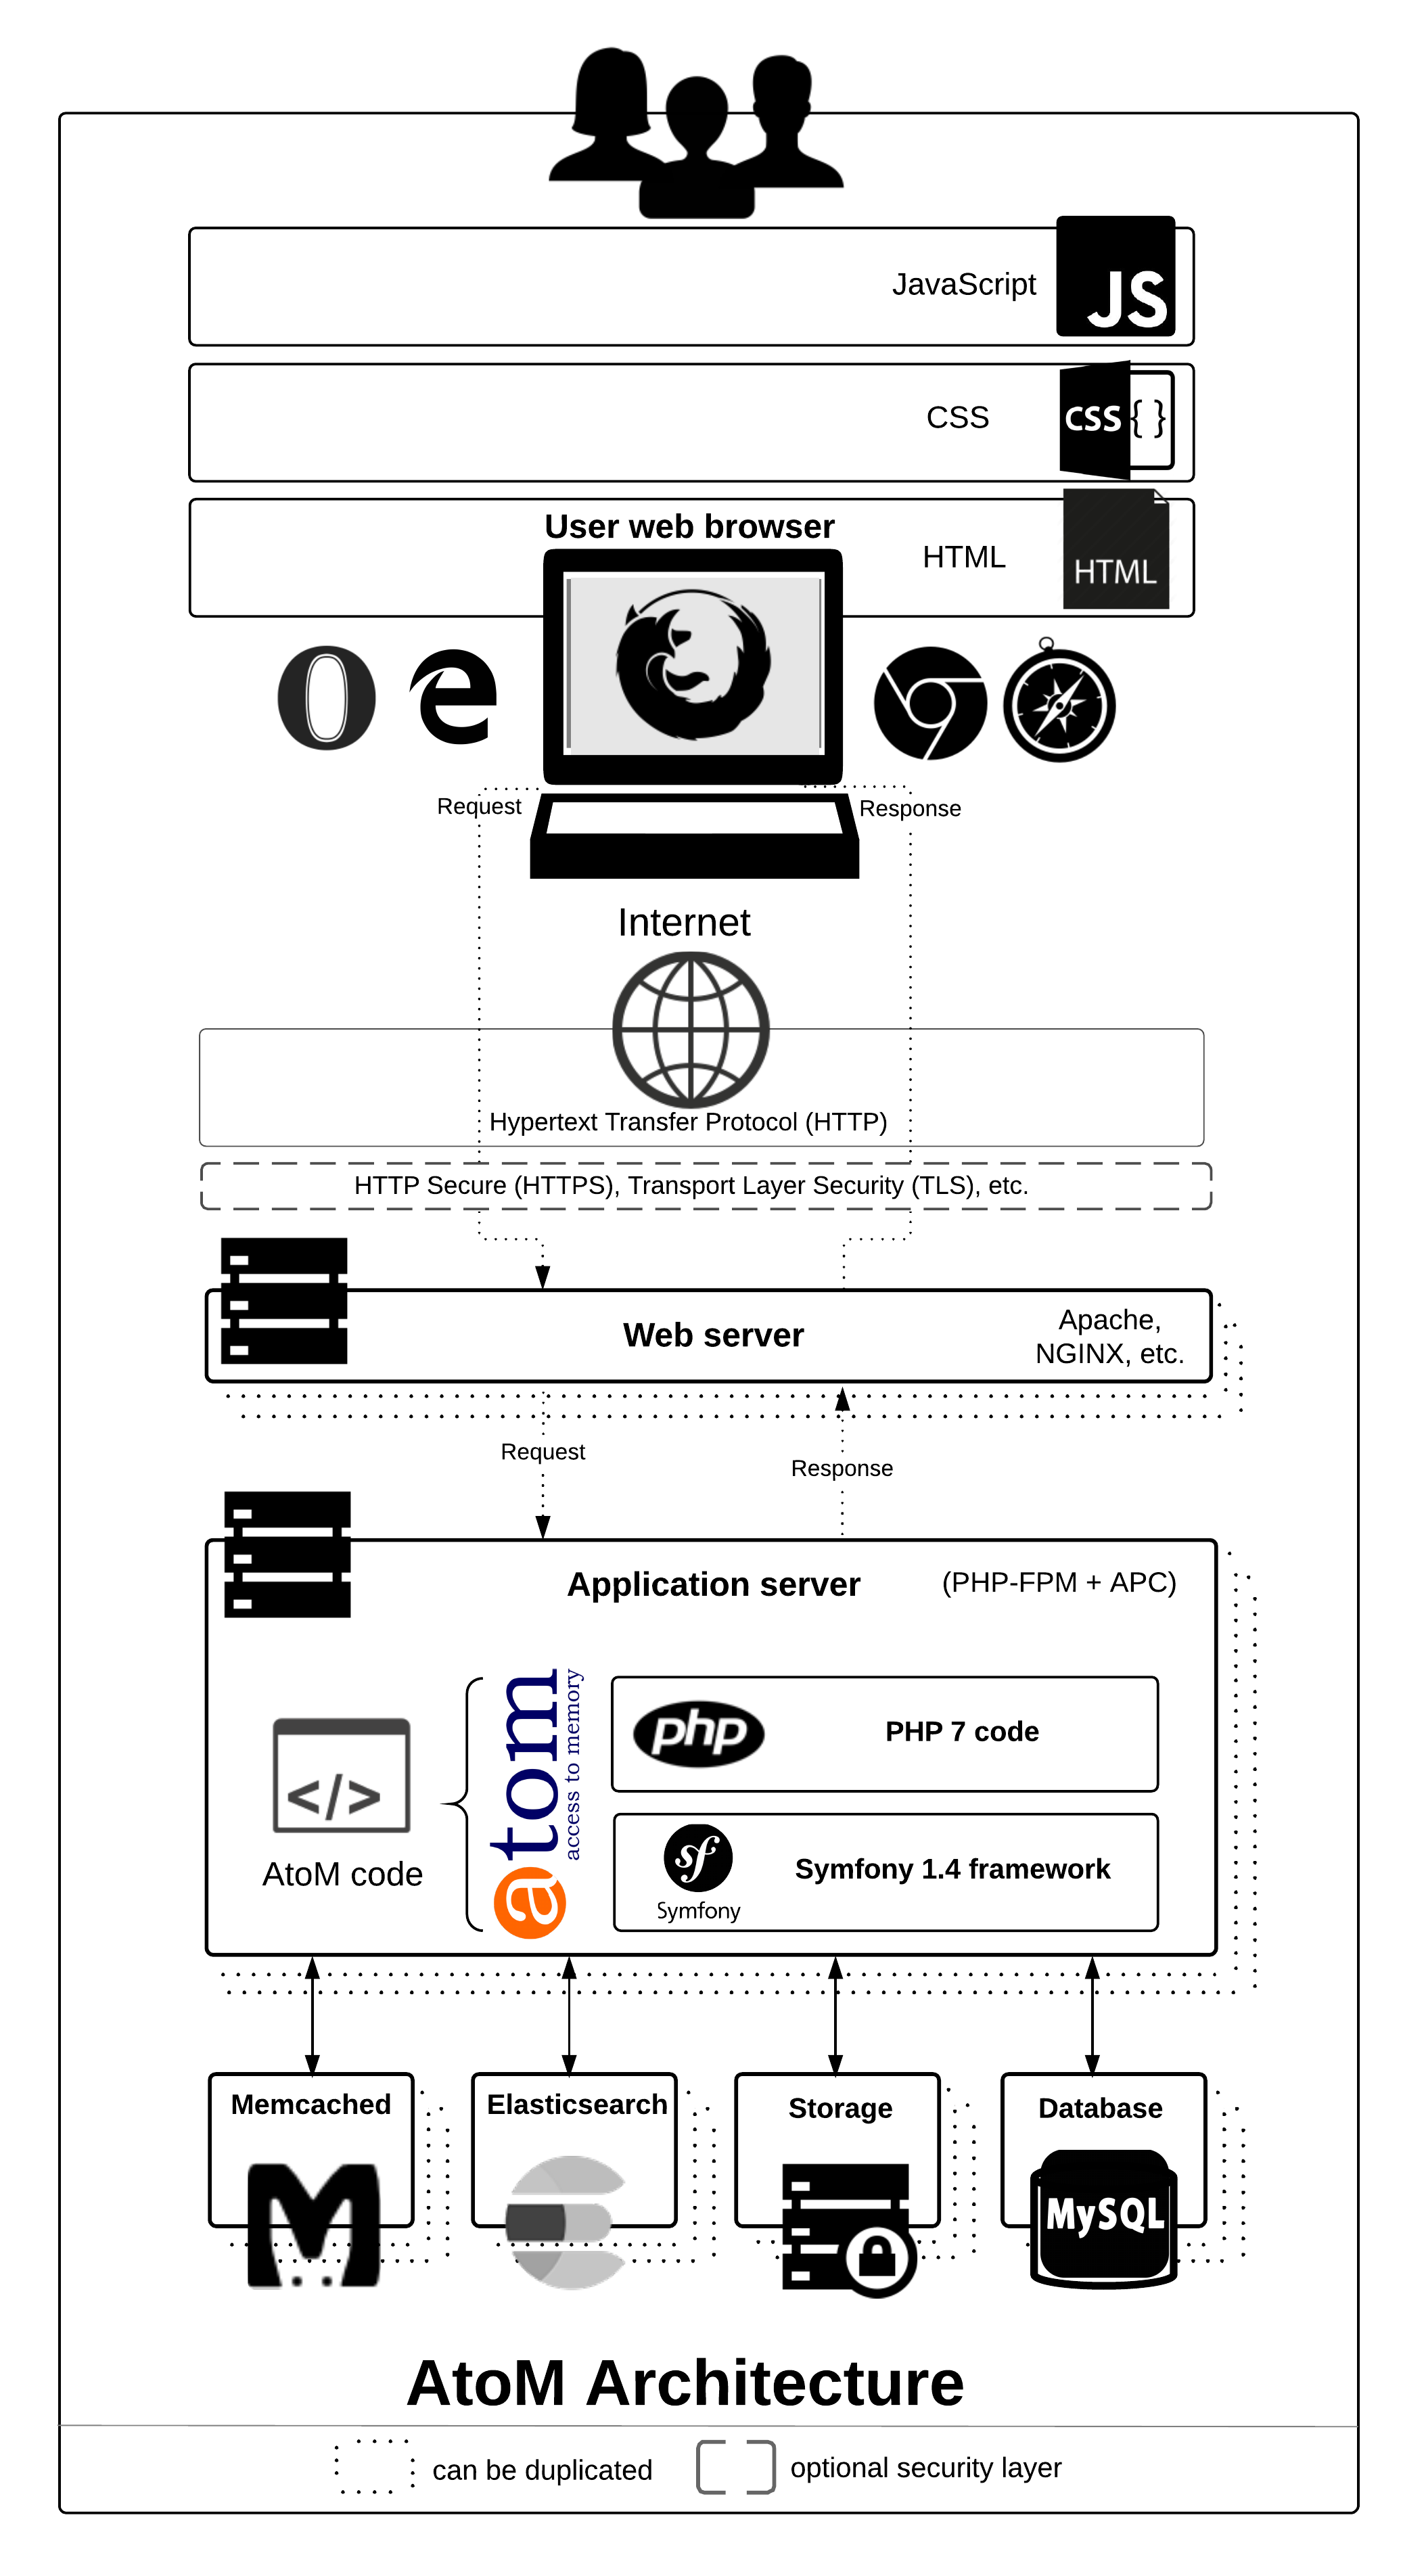
\includegraphics[max width=0.65\textwidth]{Images/what-is-atom.png}
	\end{center}  
	\begin{center}
	Рис 1. Архітектура \textbf{AtoM}.
	\end{center}
	
	\newpage
	
\textbf{AtoM складається з:} 
	
\begin{itemize}
  \item \textbf{HTML-сторінкок}, які надаються браузеру з веб-сервера. Основні два сервера, які використовуються та були протестовані розробниками є \textbf{Nginx} та \textbf{Apache}. 
  \item \textbf{Бази даних}. \textbf{MySQL (8.0)} використовується в розробці, але AtoM використовує рівень абстракції бази даних і тому потенційно сумісний з \textbf{Postgres}, \textbf{SQLite}, \textbf{SQLServer}, \textbf{Oracle}.
  
  \item \textbf{PHP-клієнт}, який керує запитами та відповідями між веб-клієнтами, логікою програми та вмістом програми, що зберігається в базі даних.
  
	\item \textbf{Symphony-Framework}, який організовує складові частини за допомогою об’єктної орієнтації та передових практик веб-дизайну.
	
	\item \textbf{Elasticsearch}. Розподілений пошуковий сервер на базі Apache Lucene, який діє як пошукова та аналітична система програми. Elasticsearch не інтегровано безпосередньо в код AtoM як бібліотеку, а як службу, розгорнуту в тій самій мережі, з якою AtoM взаємодіє через повний API REST.

\end{itemize}	

\end{large}


\section{Технічні вимоги}
Наступна інформація призначена для надання вихідної точки для налаштування вашої системи. Вона надає специфікації для розгортання «все-в-одному», зі всіма службами (тобто nginx, Percona server, ES, memcached), встановленими в одній машині.
\begin{large}

\subsection{Мінімальні вимоги}
\begin{itemize}
    \item Процесор: 2 vCPU @ 2.3 ГГц
    \item Оперативна пам'ять: 7 ГБ
    \item Місце на диску (приблизно): мінімум 50 ГБ для базової частини AtoM, додатковий простір необхідний для підтримки значної кількості цифрових об'єктів.
\end{itemize}

\subsection{Рекомендовані вимоги}
\begin{itemize}
    \item Процесор: 4 vCPU @ 2.3 ГГц
    \item Оперативна пам'ять: 16 ГБ
    \item Місце на диску (приблизно): мінімум 50 ГБ для базової частини AtoM, додатковий простір необхідний для підтримки значної кількості цифрових об'єктів.
\end{itemize}

\subsection{Обов’язкові залежності програмного забезпечення }
\begin{itemize}
    \item Веб-сервер, як-от Apache або Nginx; Artefactual.
    \item Elasticsearch версії 5.x. Elasticsearch 6.0 або новіша версія не підтримується, оскільки вони припинили підтримку деяких API, які все ще використовуються в AtoM.
    \item Java 8 (потрібна для Elasticsearch)
    \item MySQL 8.0
    \item PHP 7.4
    \item Сервер задач Gearman
\end{itemize}
Наступні PHP розширення є обов'язковими:

\begin{itemize}
    \item cURL
    \item JSON
    \item APC (також потрібен apcu-bc)
    \item PDO і PDO-MySQL
    \item XSL
\end{itemize}


\subsection{Інші залежності програмного забезпечення }

\textbf{ImageMagick} — це програмний пакет для створення, редагування, компонування або перетворення растрових зображень. Він може читати та записувати зображення в різних форматах (понад 100), включаючи DPX, EXR, GIF, JPEG, JPEG-2000, PDF, PhotoCD, PNG, Postscript, SVG і TIFF.

\textbf{ImageMagick} використовується в AtoM для створення деривативів зображень (референсного та мініатюри) з головного цифрового об’єкта, включаючи створення деривативів з багатосторінкових TIFF. ImageMagick і Ghostscript потрібні для створення одно- та багатосторінкових PDF деривативів зображень.

\textbf{Ghostscript} — це пакет програмного забезпечення на основі інтерпретатора для мов опису сторінок PostScript компанії Adobe Systems та Portable Document Format (PDF). Основними його цілями є растризація або відтворення таких мов опису сторінок для відображення або друку документів та перетворення між файлами PostScript і PDF.

\textbf{Ghostscript} використовується в AtoM разом із ImageMagick для створення одно- та багатосторінкових PDF деривативів зображень.

\textbf{FFmpeg} — це повне, кросплатформне рішення для запису, конвертування та трансляції аудіо та відео. Він включає libavcodec — провідну бібліотеку аудіо/відео кодеків.

\textbf{FFmpeg} використовується в AtoM для створення відео деривативів, включаючи створення Flash відео деривативу для перегляду у браузері.

\textbf{pdftotext} — це утиліта командного рядка з відкритим кодом для перетворення PDF файлів у звичайні текстові файли, тобто витяг даних з файлів у форматі PDF. Вона безкоштовно доступна та включена за замовчуванням у багатьох дистрибутивах Linux, а також доступна для Windows як частина Xpdf.

\textbf{Apache FOP} (Formatting Objects Processor) — це програма форматування для друку, керована об’єктами форматування XSL (XSL-FO) та незалежний від формату виведення формувач. Це програма на Java, яка зчитує дерево об'єктів форматування (FO) і відображає результат на заданий вихід.

\textbf{Apache FOP} використовується в AtoM для створення PDF-довідників.
\end{large}
\newpage
\section{Встановлення системи AtoM}
\begin{large}

\subsection{Linux}



\subsection{Windows}
Кожен елемент програмного забезпечення, \textbf{необхідний для AtoM}, сумісний з Windows. Однак слід знати, що процес може бути зовсім не простим, якщо ви не знайомі з серверними середовищами під платформою Windows.
\end{large}


\section{Конфігурація}
\begin{large}
Система \textbf{AtoM} надає багато можливостей щодо конфігурації. У цьому розділі буде описано як модерацію системи зі сторони web-сторінки, використовуючи роль адміністратора, так і ручну зміну налаштувань у внутрішніх файлам самого проекту.

\subsection{Маніпуляція налаштуваннями з веб-сторінки}

\subsection{Конфігураційні файли}

\end{large}

\section{Постскриптум}
Маємо дякувати за прочитання

\end{document}
